\documentclass[a4paper,12pt]{article}
\usepackage[utf8]{inputenc}
\usepackage[T1]{fontenc}
\usepackage[french]{babel}
\usepackage{graphicx}
\usepackage{fancyhdr}
\usepackage{xcolor}
\usepackage{titling}
\usepackage{geometry}
\usepackage{hyperref}
\geometry{margin=2.5cm}

\hypersetup{
    colorlinks=true,
    linkcolor=blue,
    urlcolor=blue,
    pdftitle={Guide d'utilisation de Spotly},
    pdfauthor={Spotly Open Source}
}

\title{\Huge \textbf{Guide d'utilisation de Spotly}}
\author{\large Spotly Open Source}
\date{\today}

\begin{document}

% Page de garde
\begin{titlepage}
    \centering
    \vspace*{3cm}
    {\Huge\bfseries Guide d'utilisation de Spotly \par}
    \vspace{2cm}
    {\Large\itshape Pour comprendre les fonctionnalités essentielles de Spotly\par}
    
\begin{figure}[h!]
    \centering
    
\includegraphics[width=0.5\textwidth]{LOGO.png}
    
\end{figure}
    \vfill
    {\large\scshape Spotly Open Source \par}
    \vspace{0.5cm}
    {\large\today\par}
\end{titlepage}

\tableofcontents
\newpage

% === Connexion à l'application ===
\section{Se connecter à l'application}

Pour se connecter à l'application Spotly, assurez-vous d’avoir un compte. Celui-ci peut vous avoir été fourni par votre organisation ou créé manuellement en vous inscrivant en cliquant sur \textbf{« Créer un compte»}.

Sur la page d’accueil, entrez votre identifiant (ou adresse email) ainsi que votre mot de passe, puis cliquez sur le bouton \textbf{« Connexion »}.

\begin{figure}[h!]
    \centering
    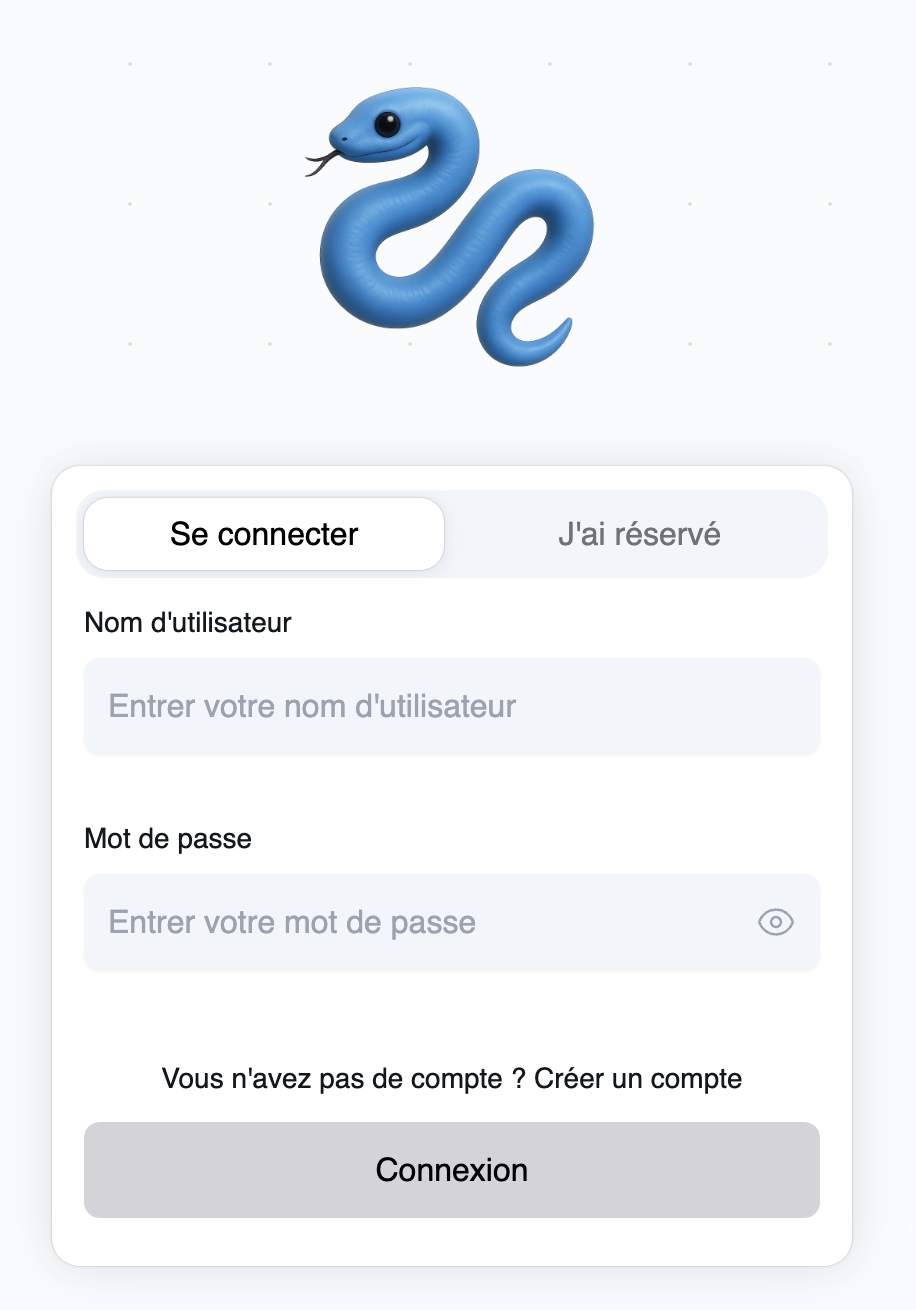
\includegraphics[width=0.5\textwidth]{UTILISATEUR/LOGIN.png}
    \caption{Interface de connexion à Spotly}
    \label{fig:login}
\end{figure}

\newpage

% === Création de compte ===
\section{Créer un compte}

Si vous n’avez pas encore de compte, vous pouvez en créer un depuis la page d’accueil en cliquant sur \textbf{« Créer un compte »}.

Renseignez les informations demandées (nom d’utilisateur, adresse email, mot de passe), puis validez en cliquant sur \textbf{« Créer mon compte »}.

\begin{figure}[h!]
    \centering
    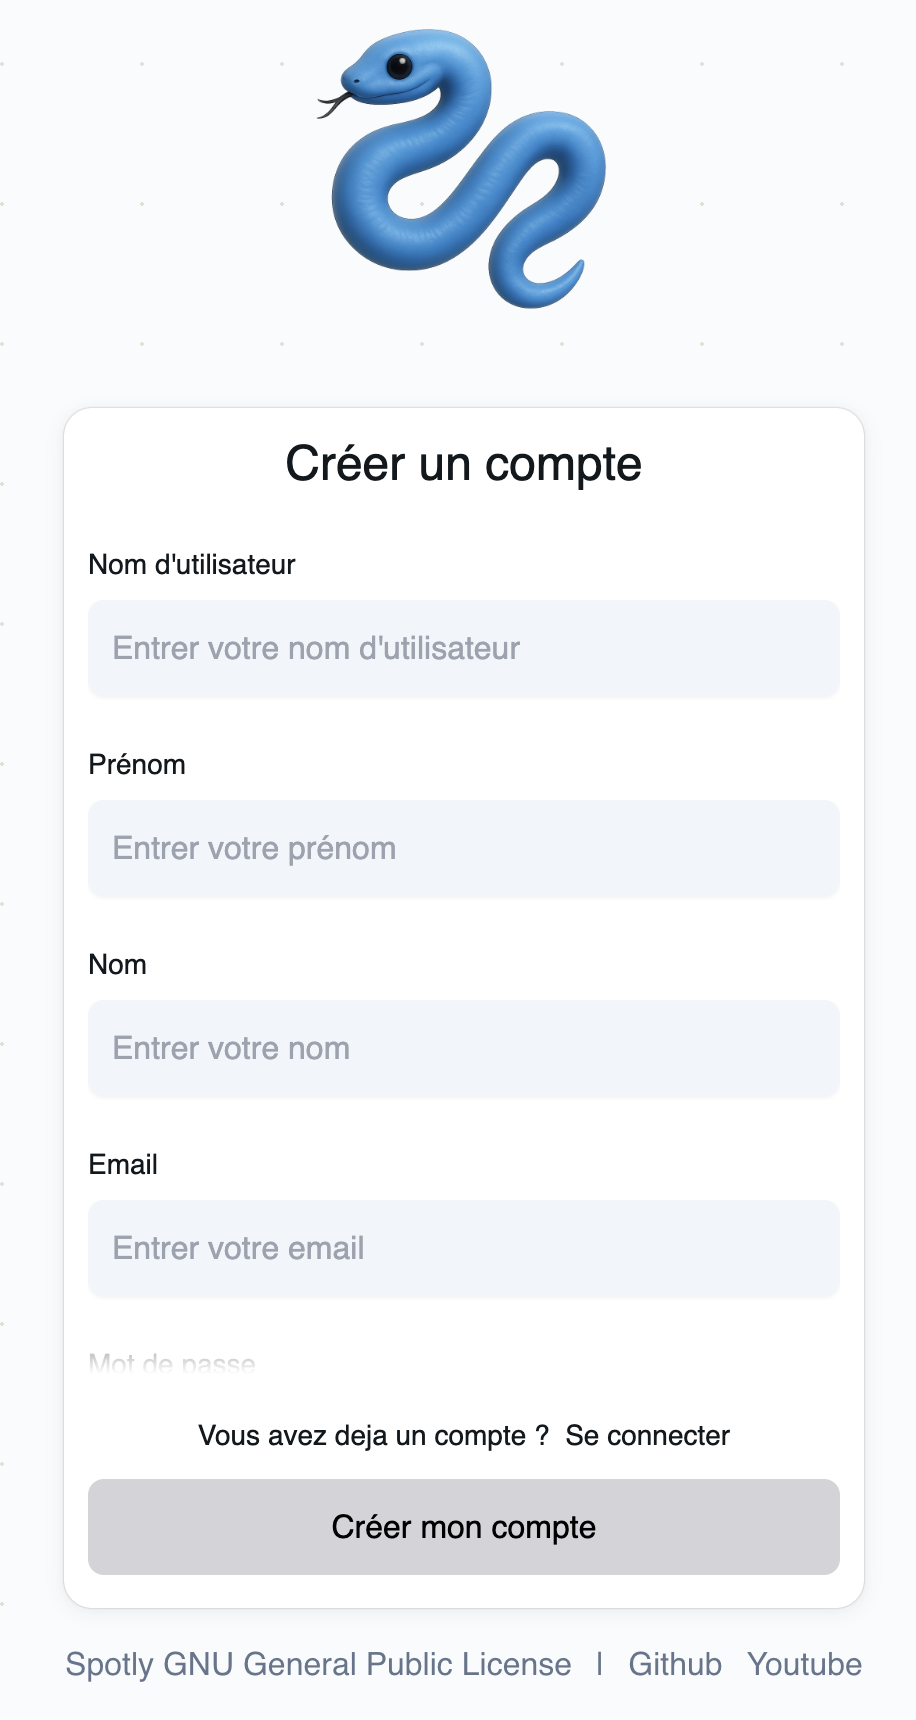
\includegraphics[width=0.5\textwidth]{UTILISATEUR/REGISTER.png}
    \caption{Formulaire d’inscription}
    \label{fig:register}
\end{figure}

\newpage

% === Recherche de ressource ===
\section{Rechercher une ressource}

Une fois sur la page d’accueil, vous pouvez  \textbf{réserver une ressource}. Une interface vous permet de configurer une recherche.

\begin{itemize}
    \item Choisissez le \textbf{site} et la \textbf{catégorie} de ressource souhaitée.
    \item (Optionnel) sélectionnez une ressource spécifique.
    \item Indiquez les dates et heures de début et de fin.
\end{itemize}

\begin{figure}[h!]
    \centering
    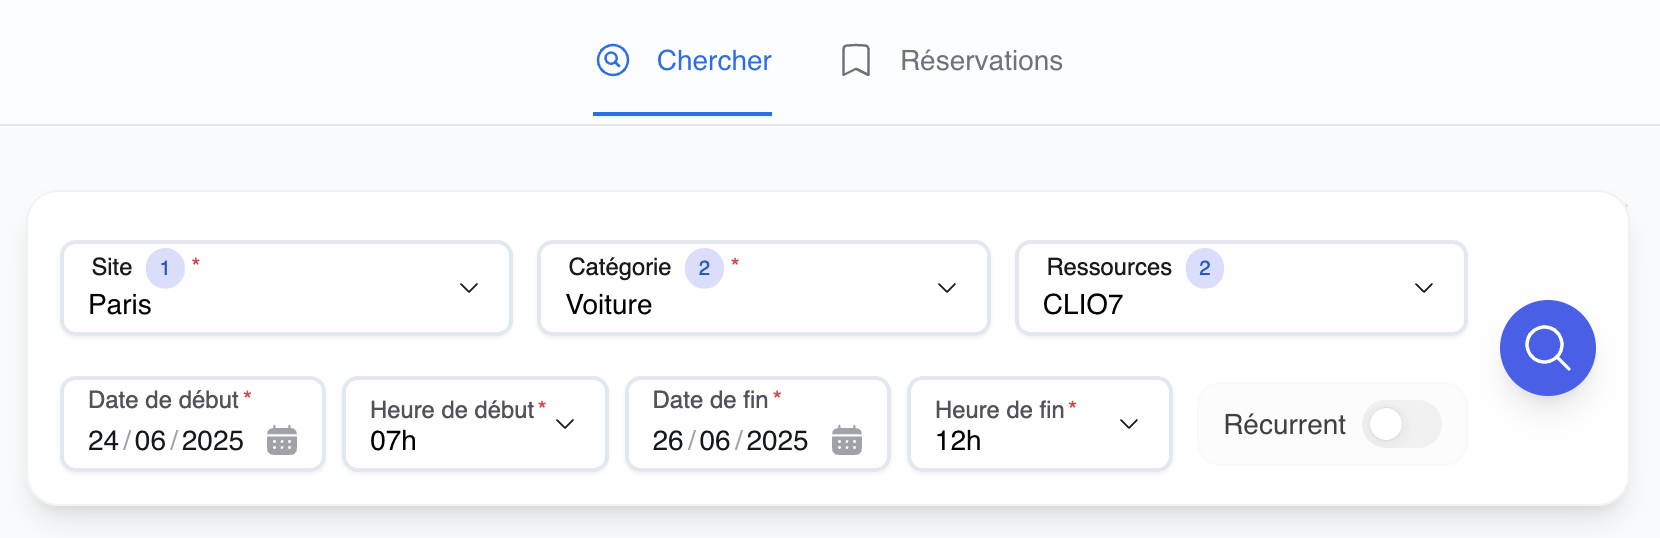
\includegraphics[width=0.75\textwidth]{UTILISATEUR/SEARCH_WITH_PARAMETERS.png}
    \caption{Recherche avec critères de réservation}
    \label{fig:search-parameters}
\end{figure}

Lancez la recherche en cliquant sur l’icône de loupe. Vous pouvez réserver sur plusieurs crénaux en cliquant sur \textbf{«Récurrent»}, par jour ou par semaine, jusqu'à une date limite.

\begin{figure}[h!]
    \centering
    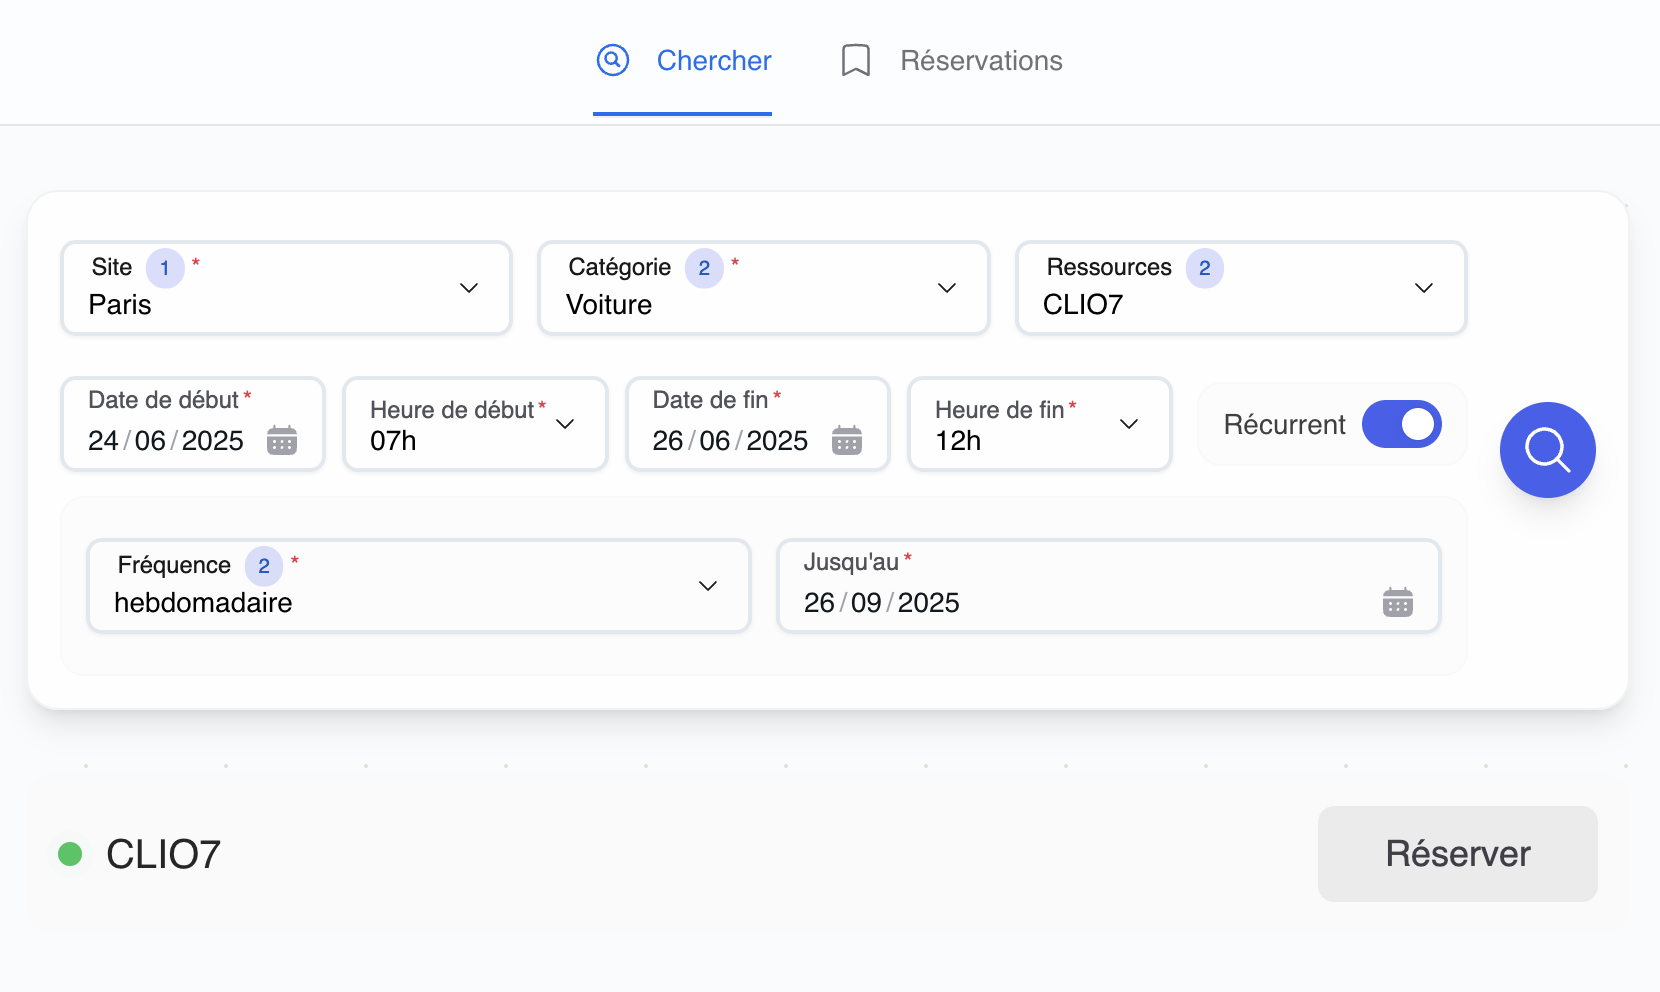
\includegraphics[width=0.75\textwidth]{UTILISATEUR/SEARCH_WITH_RESULTS.png}
    \caption{Résultats de recherche}
    \label{fig:search-results}
\end{figure}

\newpage

% === Réserver une ressource ===
\section{Réserver une ressource}

Après avoir trouvé une ressource disponible, vous avez deux possibilités :

\begin{itemize}
    \item \textbf{Réserver} : réservation directe sans validation.
    \item \textbf{Demander} : requiert l’approbation d’un manager.
\end{itemize}

\begin{figure}[h!]
    \centering
    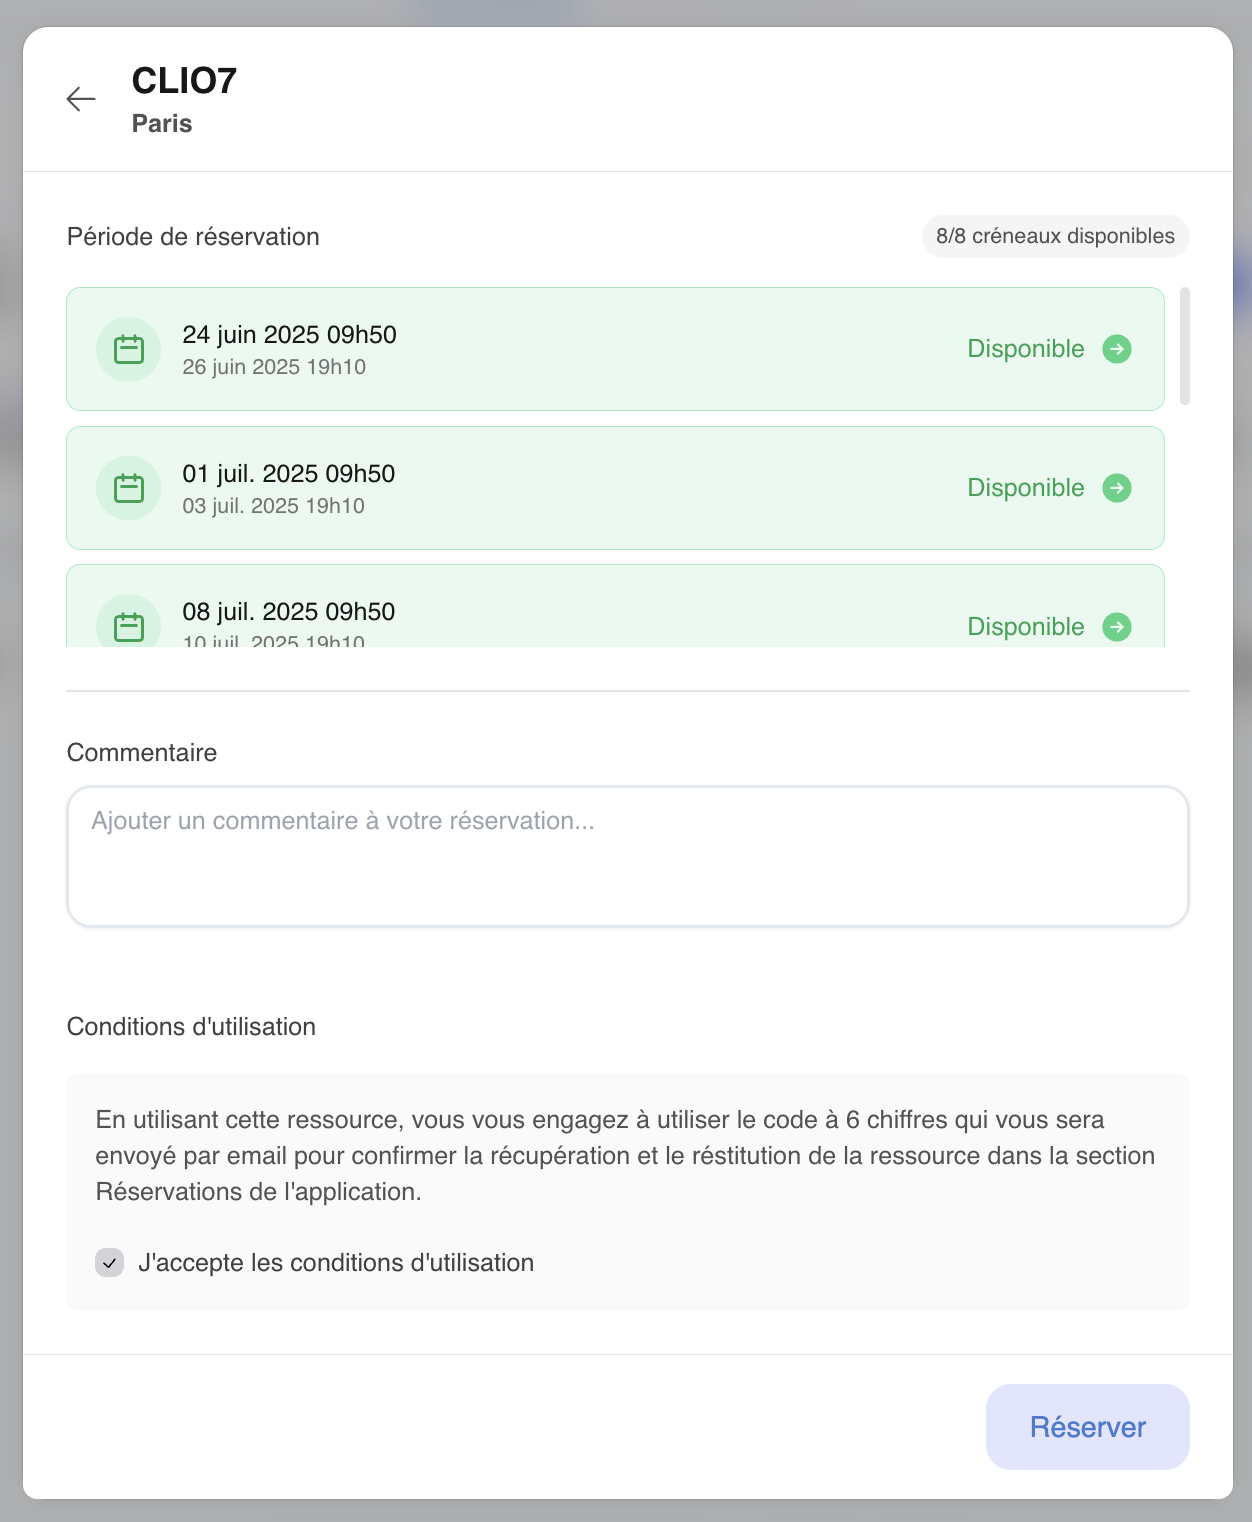
\includegraphics[width=0.5\textwidth]{UTILISATEUR/BOOK_RECAP.png}
    \caption{Récapitulatif avant réservation}
    \label{fig:book-recap}
\end{figure}

\newpage

% === Suivre l'état de la réservation ===
\section{Suivre l'état d'une réservation}

Les réservations peuvent avoir plusieurs états :

\begin{itemize}
    \item \textbf{Acceptée} : validée automatiquement ou par un manager.
    \item \textbf{En cours} : la ressource est en votre possession.
    \item \textbf{Terminée} : la période de réservation est passée.
\end{itemize}

\begin{figure}[h!]
    \centering
    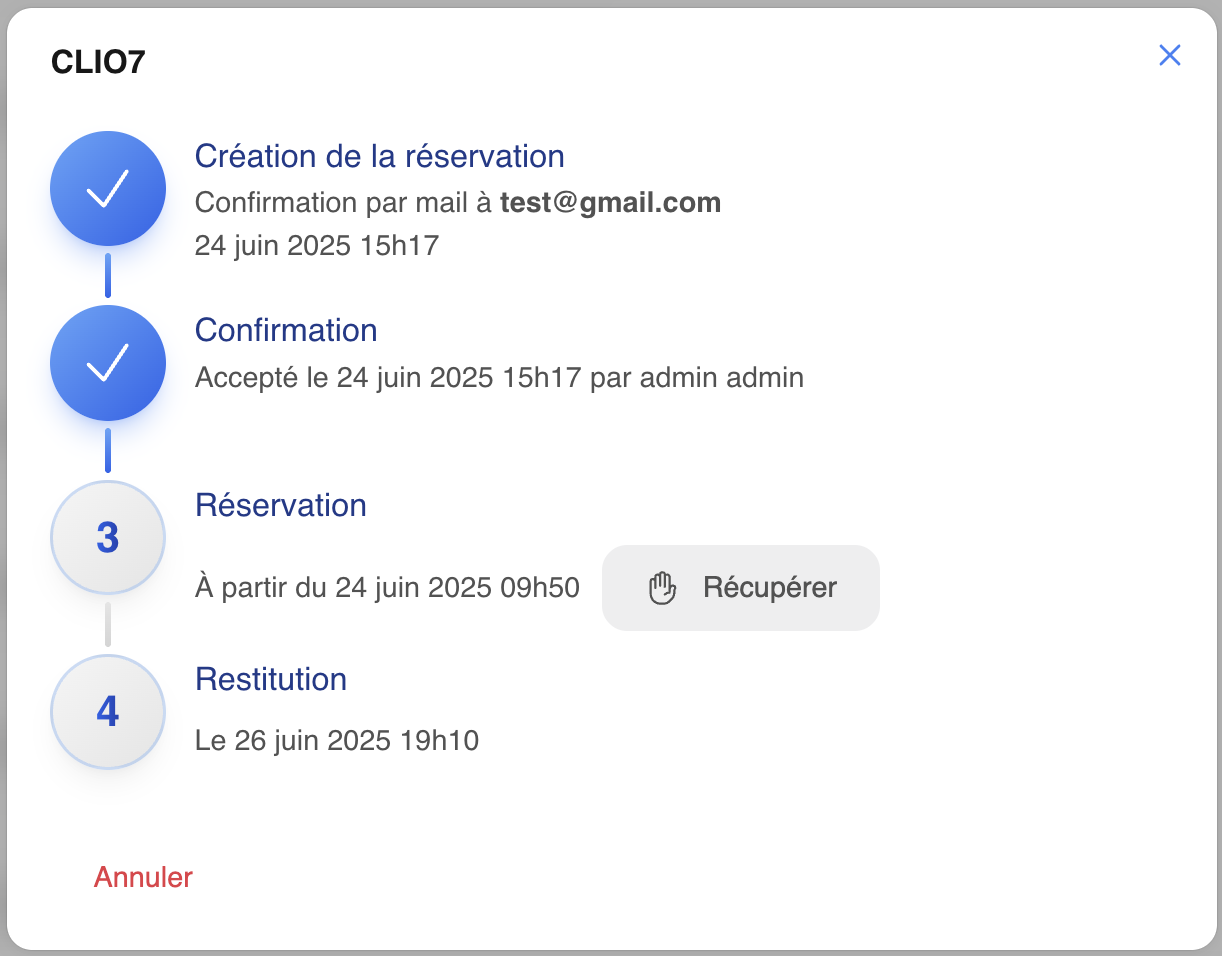
\includegraphics[width=0.65\textwidth]{UTILISATEUR/BOOK_MODAL_ACCEPTED.png}
    \caption{Réservation acceptée}
\end{figure}

\begin{figure}[h!]
    \centering
    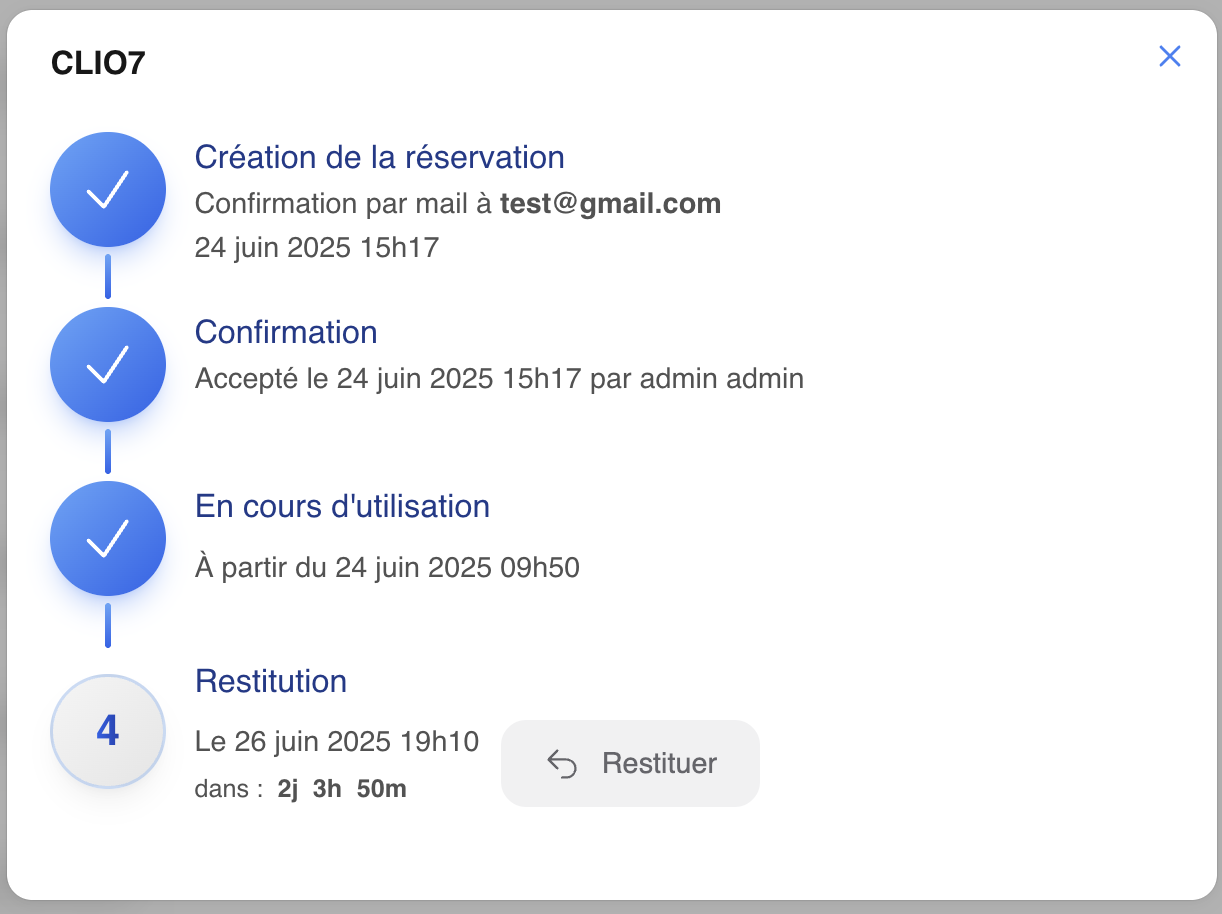
\includegraphics[width=0.65\textwidth]{UTILISATEUR/BOOK_MODAL_USED.png}
    \caption{Réservation en cours}
\end{figure}

\begin{figure}[h!]
    \centering
    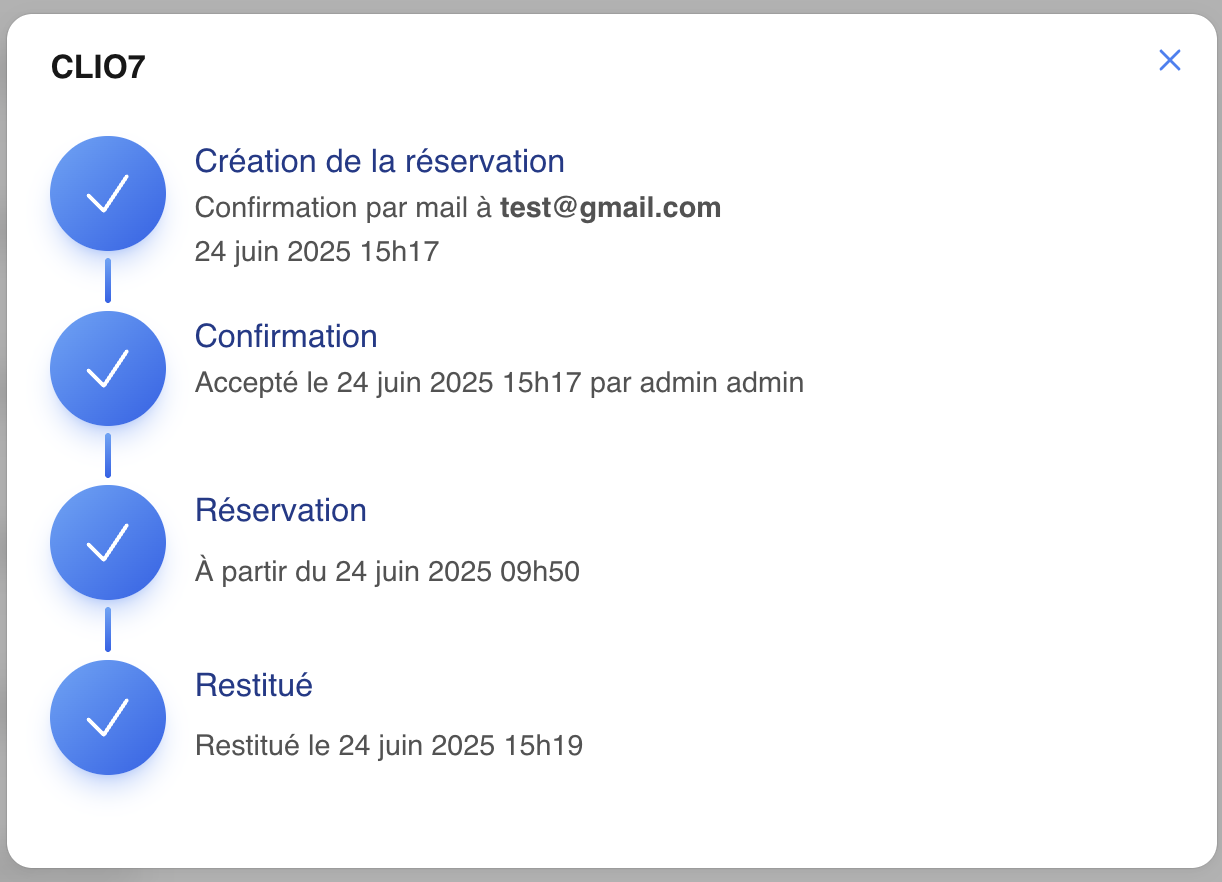
\includegraphics[width=0.65\textwidth]{UTILISATEUR/BOOK_MODAL_ENDED.png}
    \caption{Réservation terminée}
\end{figure}

\newpage

% === Consulter mes réservations ===
\section{Consulter mes réservations}

L’onglet \textbf{« Réservations »} vous permet de voir l’ensemble de vos réservations passées, en cours ou planifiées.

\begin{figure}[h!]
    \centering
    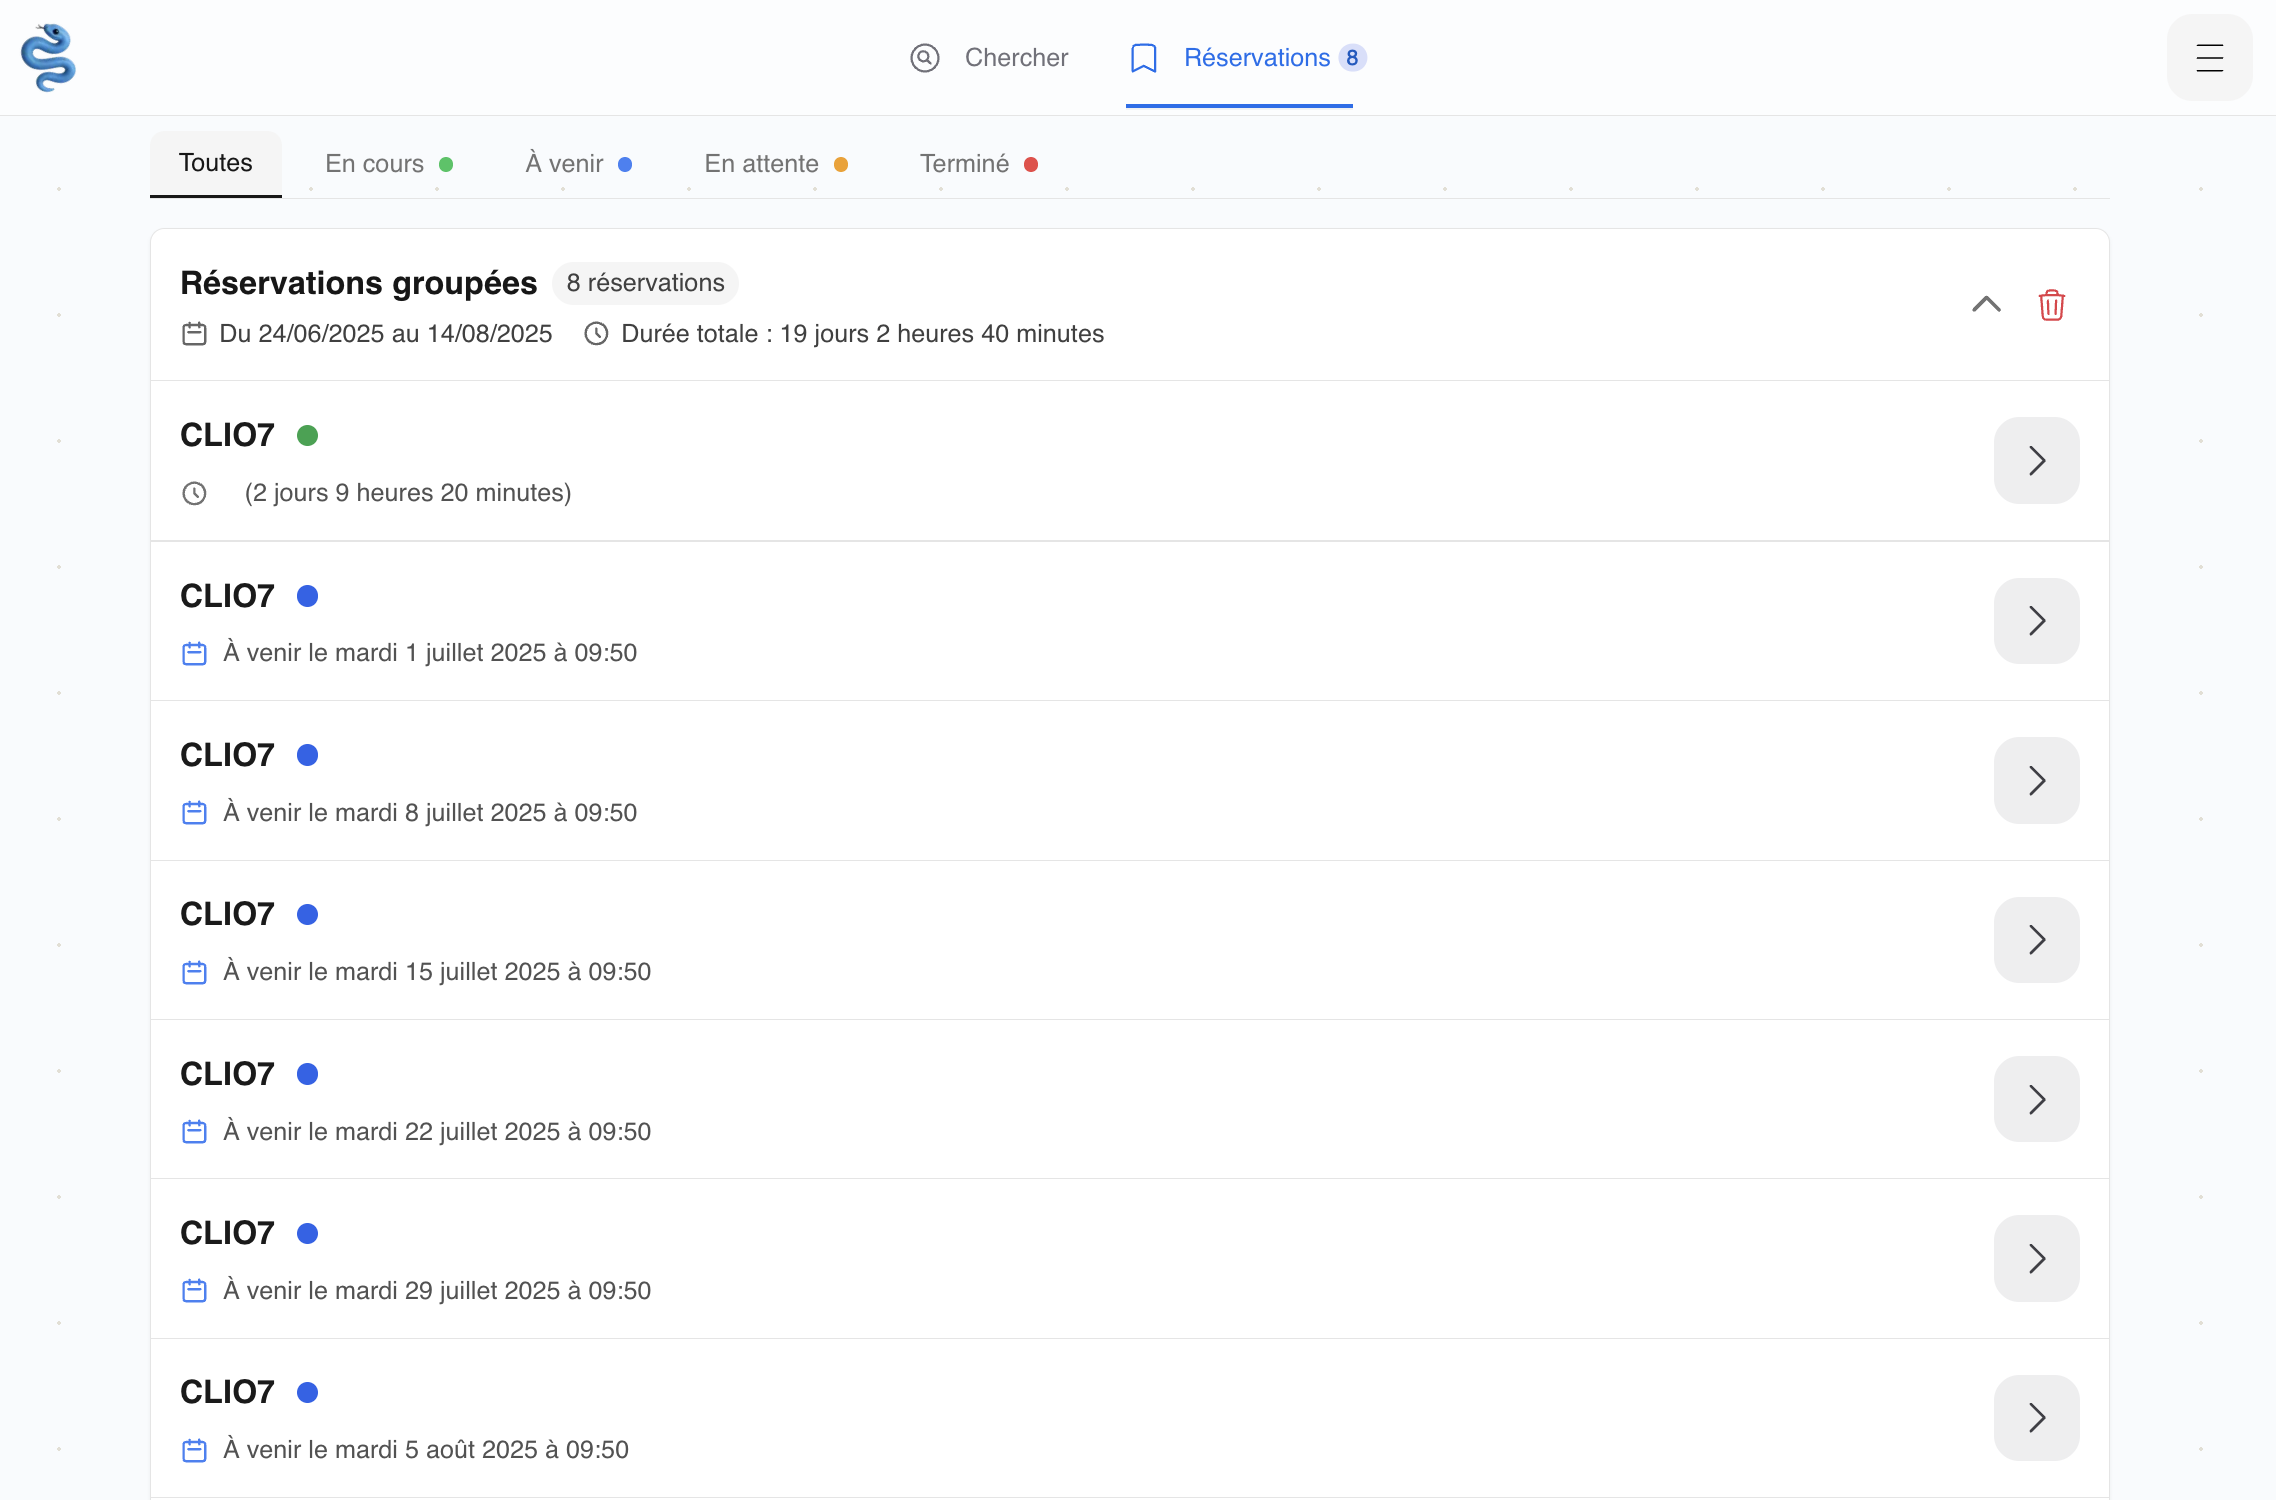
\includegraphics[width=0.8\textwidth]{UTILISATEUR/BOOKS_LISTINGS.png}
    \caption{Liste des réservations utilisateur}
    \label{fig:book-list}
\end{figure}

\newpage

% === Annuler une réservation ===
\section{Annuler une réservation}

Pour annuler une réservation :

\begin{enumerate}
    \item Allez dans l’onglet \textbf{Réservations}.
    \item Cliquez sur la réservation souhaitée.
    \item Cliquez sur \textbf{« Annuler »} puis {« Confirmer l'annulation »}.
\end{enumerate}

\begin{figure}[h!]
    \centering
    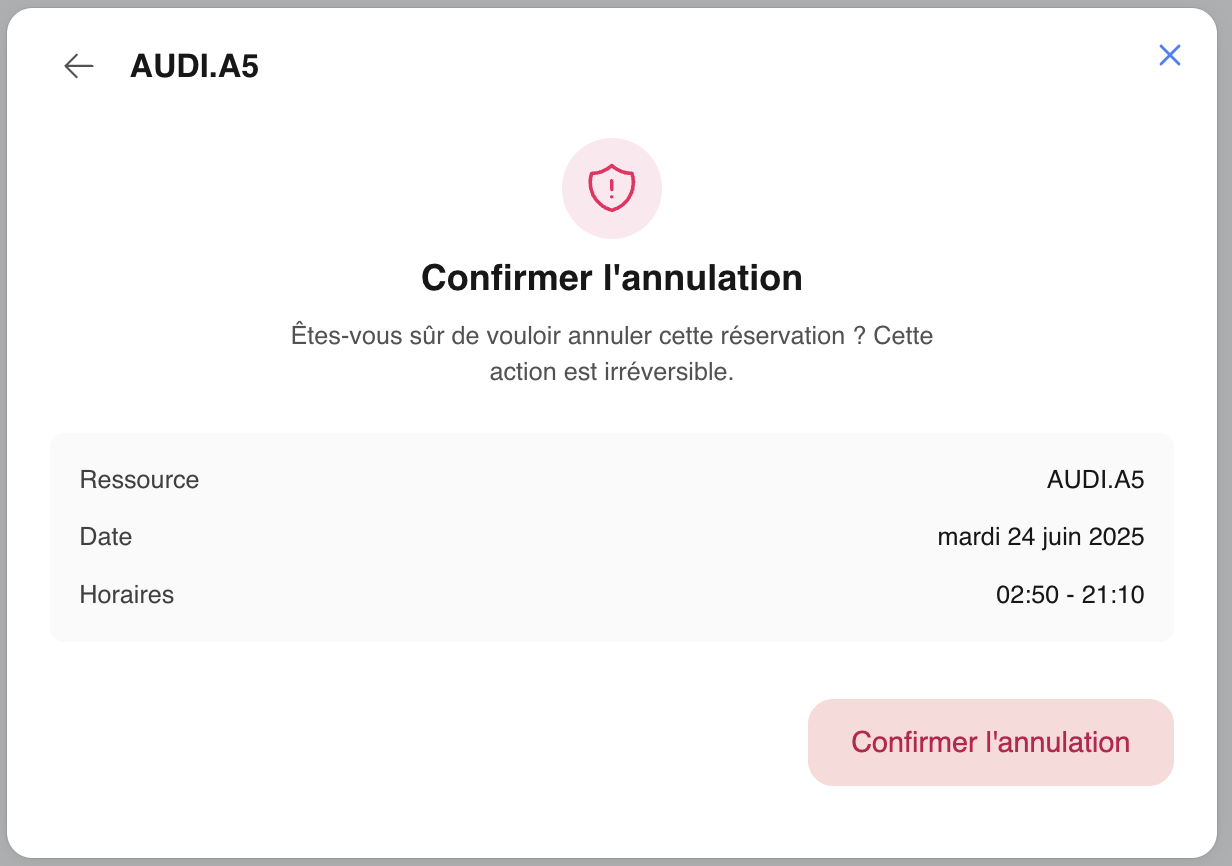
\includegraphics[width=0.5\textwidth]{UTILISATEUR/CANCEL_BOOK_CONFIRM.png}
    \caption{Confirmation d’annulation d’une réservation}
\end{figure}

Il est aussi possible d’annuler les réservations groupée d’un seul coup :

\begin{figure}[h!]
    \centering
    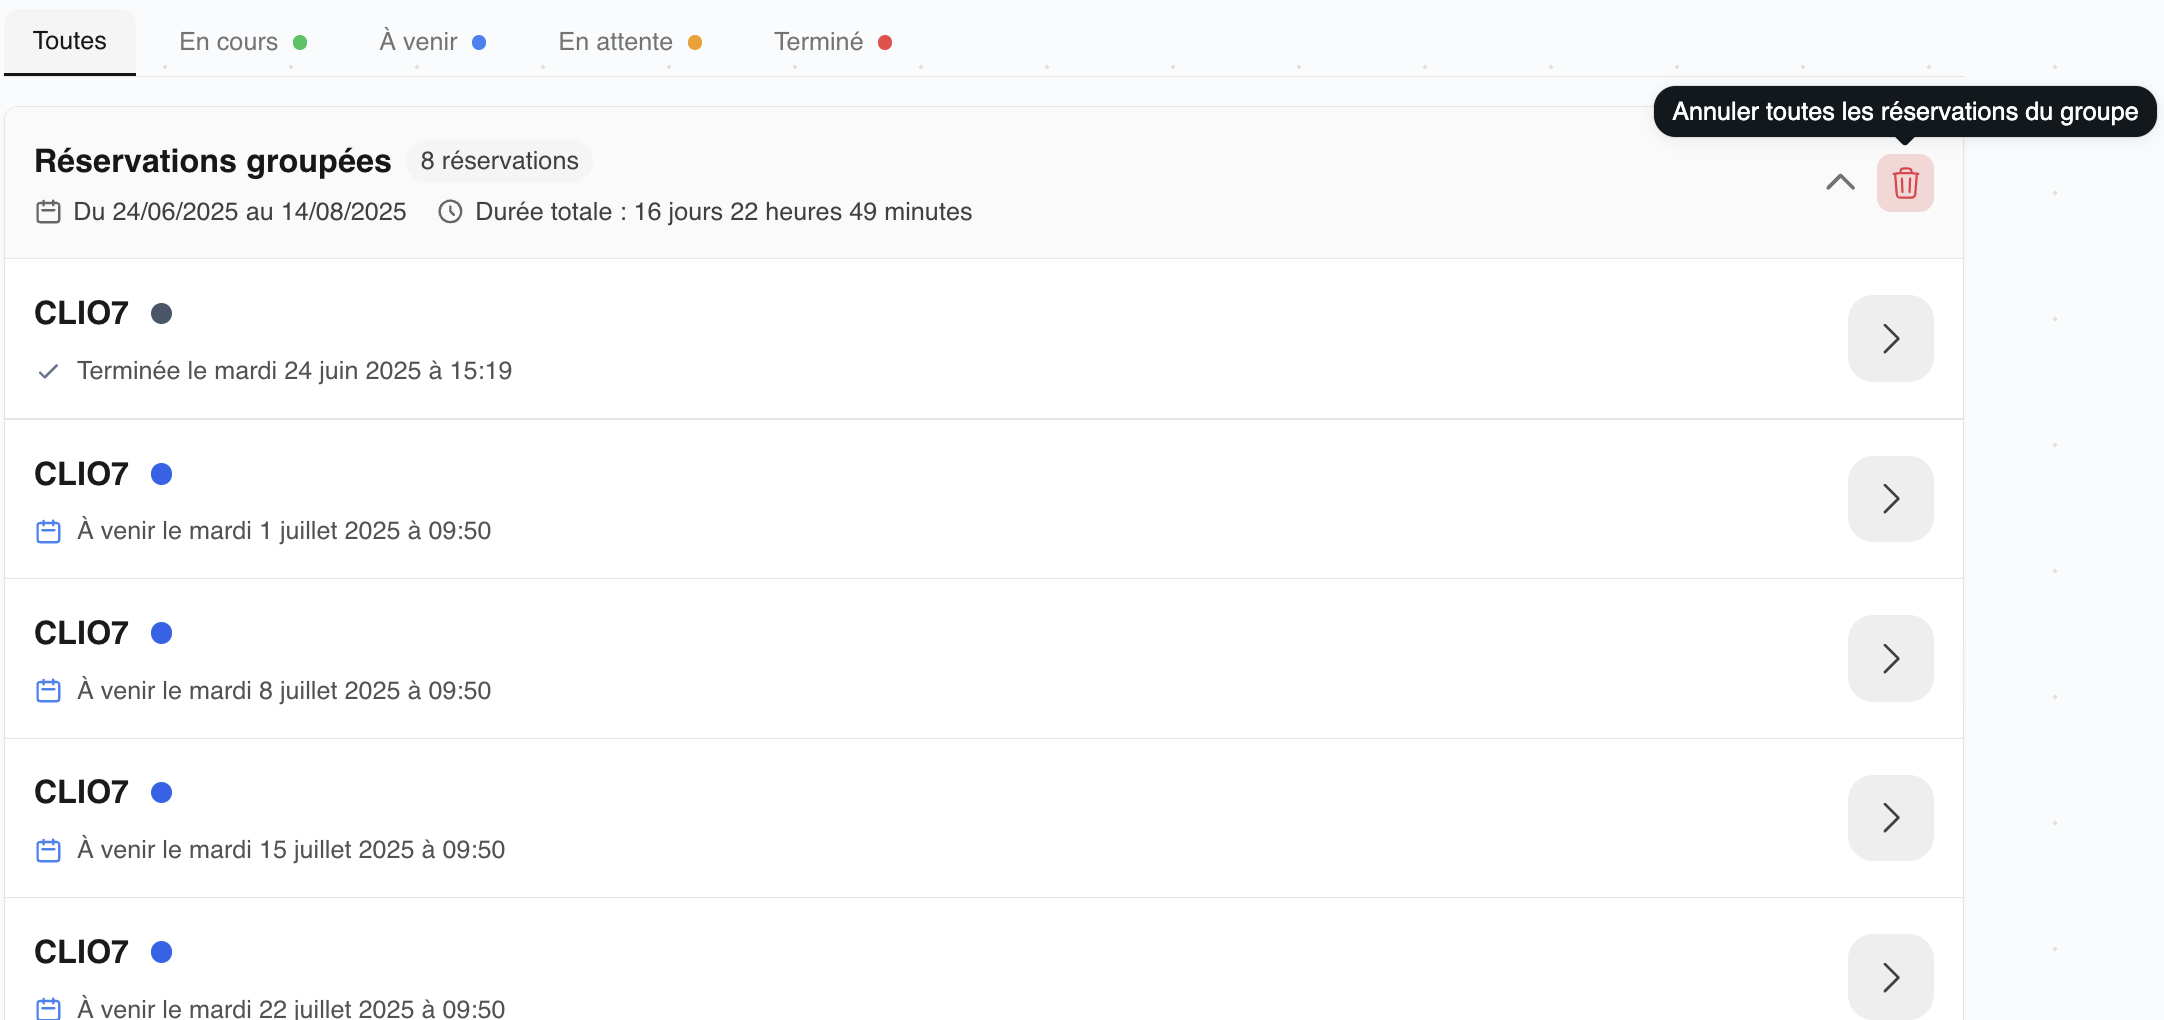
\includegraphics[width=0.5\textwidth]{UTILISATEUR/CANCEL_BOOKS_GROUP.png}
    \caption{Sélection de plusieurs réservations}
\end{figure}

\begin{figure}[h!]
    \centering
    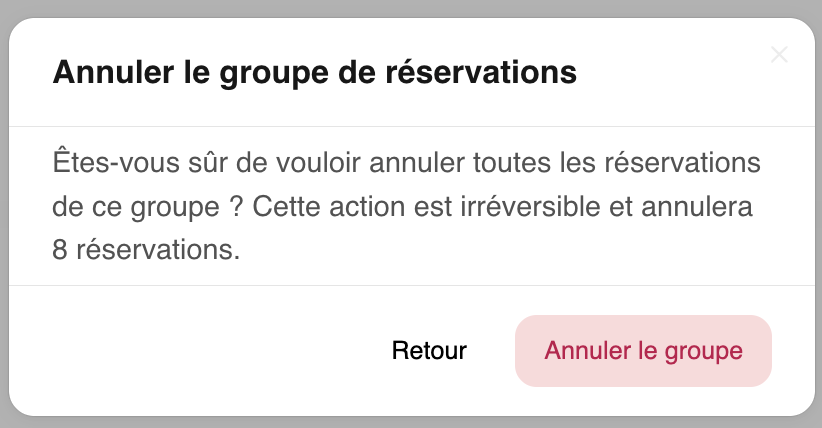
\includegraphics[width=0.5\textwidth]{UTILISATEUR/CANCEL_BOOKS_GROUP_CONFIRM.png}
    \caption{Confirmation de l’annulation groupée}
\end{figure}




\end{document}
